\documentclass[11pt]{scrreprt}
\usepackage[left=25mm,right=25mm,top=25mm,bottom=25mm]{geometry}
\usepackage[utf8]{inputenc}
\usepackage[ngerman]{babel}
\usepackage{float}
\usepackage{graphicx}
\usepackage{textcomp, gensymb}
\usepackage{caption}
\usepackage{xcolor}
\usepackage{url}
\usepackage{hyperref}
\usepackage{varioref}
\usepackage{mathtools}
\usepackage{amssymb}
\usepackage{siunitx}
\usepackage[version=4]{mhchem}
\usepackage{cleveref}
\usepackage{pdfpages}
\usepackage{tikz}
% Schönere Tabellen
\usepackage{booktabs}
% Plotten, Tabellen und vieles mehr
\usepackage{pgfplots}
\pgfplotsset{compat=1.16}


\begin{document}

% Verhindert die Seitennummerierung auf der Titelseite
\pagenumbering{gobble}

%--------Deckblatt Versuchsprotokoll----------%
% Der input-Befehl lädt den LaTeX-Code aus der angegeben Datei und fügt ihn an dieser Stelle ein.
% Hier müsst ihr dafür sorgen, dass die entsprechend nicht genutzte Version mit einem % auskommentiert ist
% Hier bitte ausfüllen:
\newcommand{\praktikum}{} % Praktikum
\newcommand{\semester}{} % Semester
\newcommand{\wochentag}{} % Wochentag-Gruppe
\newcommand{\gruppennummer}{} % Gruppennummer
\newcommand{\nachnameeins}{} % Nachname1
\newcommand{\nachnamezwei}{} % Nachname2
\newcommand{\vornameeins}{} % Vorname1
\newcommand{\vornamezwei}{} % Vorname2
\newcommand{\email}{} % E-Mail Adressen
\newcommand{\versuch}{} % Versuch
\newcommand{\fehlerrechnung}{} % Fehlerrechnung
\newcommand{\betreuer}{} % Betreuer:in
\newcommand{\durchfuehrungsdatum}{} % Durchgeführt am
\newcommand{\abgabedatumeins}{} % 1. Abgabe am:
\newcommand{\abgabedatumzwei}{} % 2. Abgabe am:
%%%%%%%%%%%%%%%%%%%%%%%%%%%%%%%%%%%%%%%%%%%%%%%%%%%%%%%%%%%%%%%%%%%%%%%%%%%%%%%%%%%%%%%%%
\begin{tikzpicture}[remember picture,overlay]
    \node at (current page.center) {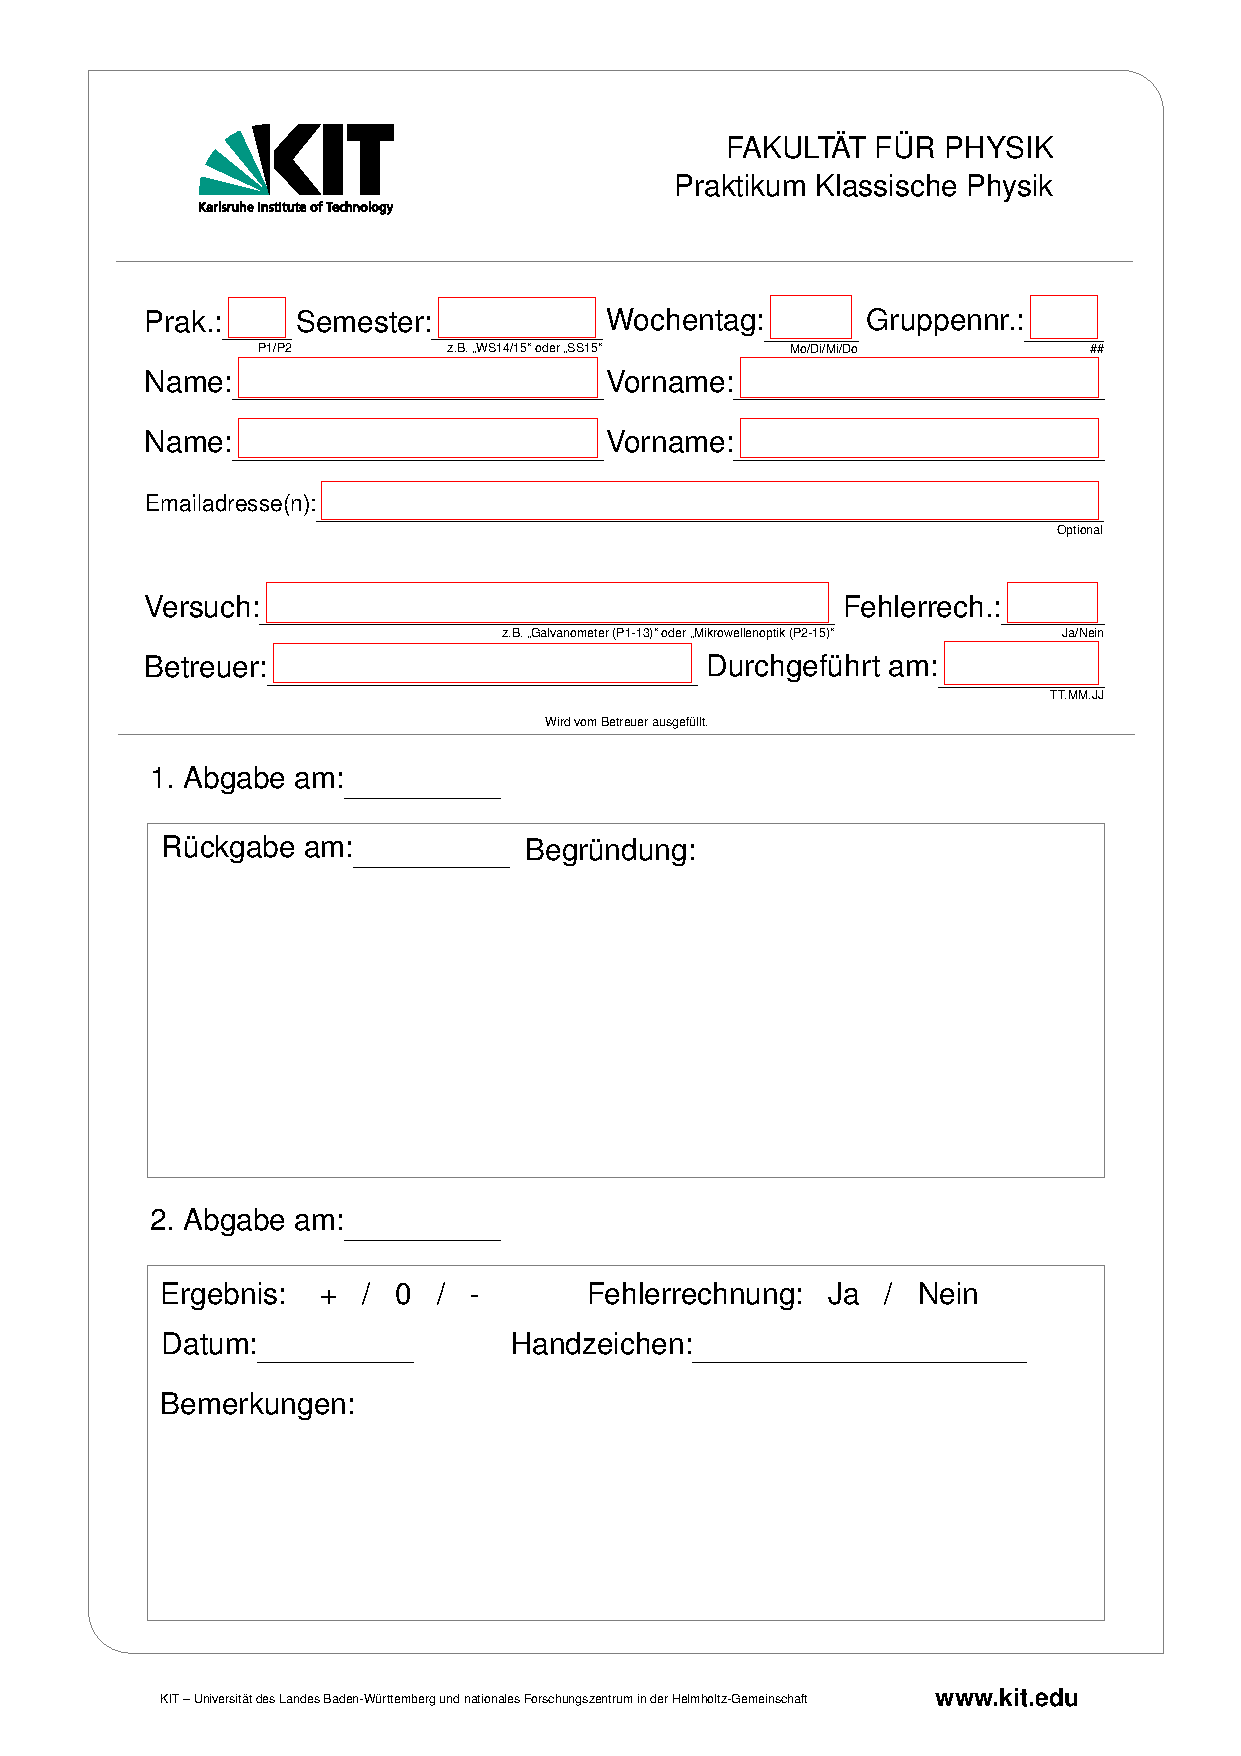
\includegraphics[page=1]{include/DeckblattP1P2.pdf}};
    \begin{scope}[shift={(current page.south west)},every node/.style={anchor=base west}]
        % Grid to help find the positions (remove in final version)
        %\draw [help lines] (0,0) grid (current page.north east);
        %\draw [help lines,thick] (0,0) grid [step=5cm] (current page.north east);
        %
        \node at (3.95cm,24.15cm) {\Large{\praktikum}}; % Praktikum:
        \node at (7.5cm,24.15cm) {\Large{\semester}}; % Semester:
        \node at (13.2cm,24.15cm){\Large{\wochentag}}; % Wochentag-Gruppe:
        \node at (17.6cm,24.15cm){\Large{\gruppennummer}};% Gruppennummer:
        \node at (4cm,23.1cm){\Large{\nachnameeins}}; % Nachname1:
        \node at (4cm,22.1cm){\Large{\nachnamezwei}}; % Nachname2:
        \node at (12.5cm,23.1cm){\Large{\vornameeins}}; % Vorname1:
        \node at (12.5cm,22.1cm){\Large{\vornamezwei}}; % Vorname2:
        \node at (5.4cm,21.1cm){\Large{\email}}; % E-Mail Adressen:
        \node at (4.5cm,19.3cm){\Large{\versuch}}; %Versuch:
        \node at (17.1cm,19.3cm){\Large{\fehlerrechnung}}; % Fehlerrechnung:
        \node at (4.55cm,18.3cm){\Large{\betreuer}}; % Betreuer:in:
        \node at (16cm,18.3cm){\Large{\durchfuehrungsdatum}}; % Durchgeführt am:
        \node at (5.9cm,16.4cm){\Large{\abgabedatumeins}}; % 1. Abgabe am:
        \node at (6cm,15.2cm){\Large{}}; %Rückgabe am:
        \node at (5.8cm,8.9cm){\Large{\abgabedatumzwei}}; % 2. Abgabe am:
    \end{scope}
\end{tikzpicture}
% This information will appear embed into the PDF file as meta data
\hypersetup{
  pdftitle    = {\praktikum\hspace{0.2222em}Protokoll - \versuch},
  pdfsubject  = {Protokoll des Versuchs \versuch\hspace{0.2222em}vom \durchfuehrungsdatum},
  pdfauthor   = {\vornameeins\hspace{0.2222em}\nachnameeins\hspace{0.2222em}und\hspace{0.2222em}\vornamezwei\hspace{0.2222em}\nachnamezwei\hspace{0.2222em}(Gruppe \wochentag\gruppennummer)},
  pdfkeywords = {KIT, Physik, Praktikum, Protokoll, \praktikum, \versuch, \semester, \vornameeins\hspace{0.2222em}\nachnameeins, \vornamezwei\hspace{0.2222em}\nachnamezwei} ,
  pdfcreator  = {pdflatex},
  pdfproducer = {LaTeX with hyperref}
}
%% Hier bitte ausfüllen:
\newcommand{\praktikum}{} % Praktikum P3/P4
\newcommand{\gruppennummer}{} % Gruppennummer
\newcommand{\gruppentag}{} % Gruppentag
\newcommand{\semester}{} % Semester
\newcommand{\versuch}{} % Versuch
\newcommand{\nameeins}{} % Name1 (Vor und Nachname)
\newcommand{\emaileins}{} % E-Mail 1
\newcommand{\namezwei}{} % Name2 (Vor und Nachname)
\newcommand{\emailzwei}{} % E-Mail 2
\newcommand{\assistent}{} % Assistent:in
\newcommand{\durchfuehrungsdatum}{} % Durchgeführt am
\newcommand{\abgabedatum}{} % Protokollabgabe am:
%%%%%%%%%%%%%%%%%%%%%%%%%%%%%%%%%%%%%%%%%%%%%%%%%%%%%%%%%%%%%%%%%%%%%%%%%%%%%%%%%%%%%%%%%
\begin{tikzpicture}[remember picture,overlay]
    \node at (current page.center) {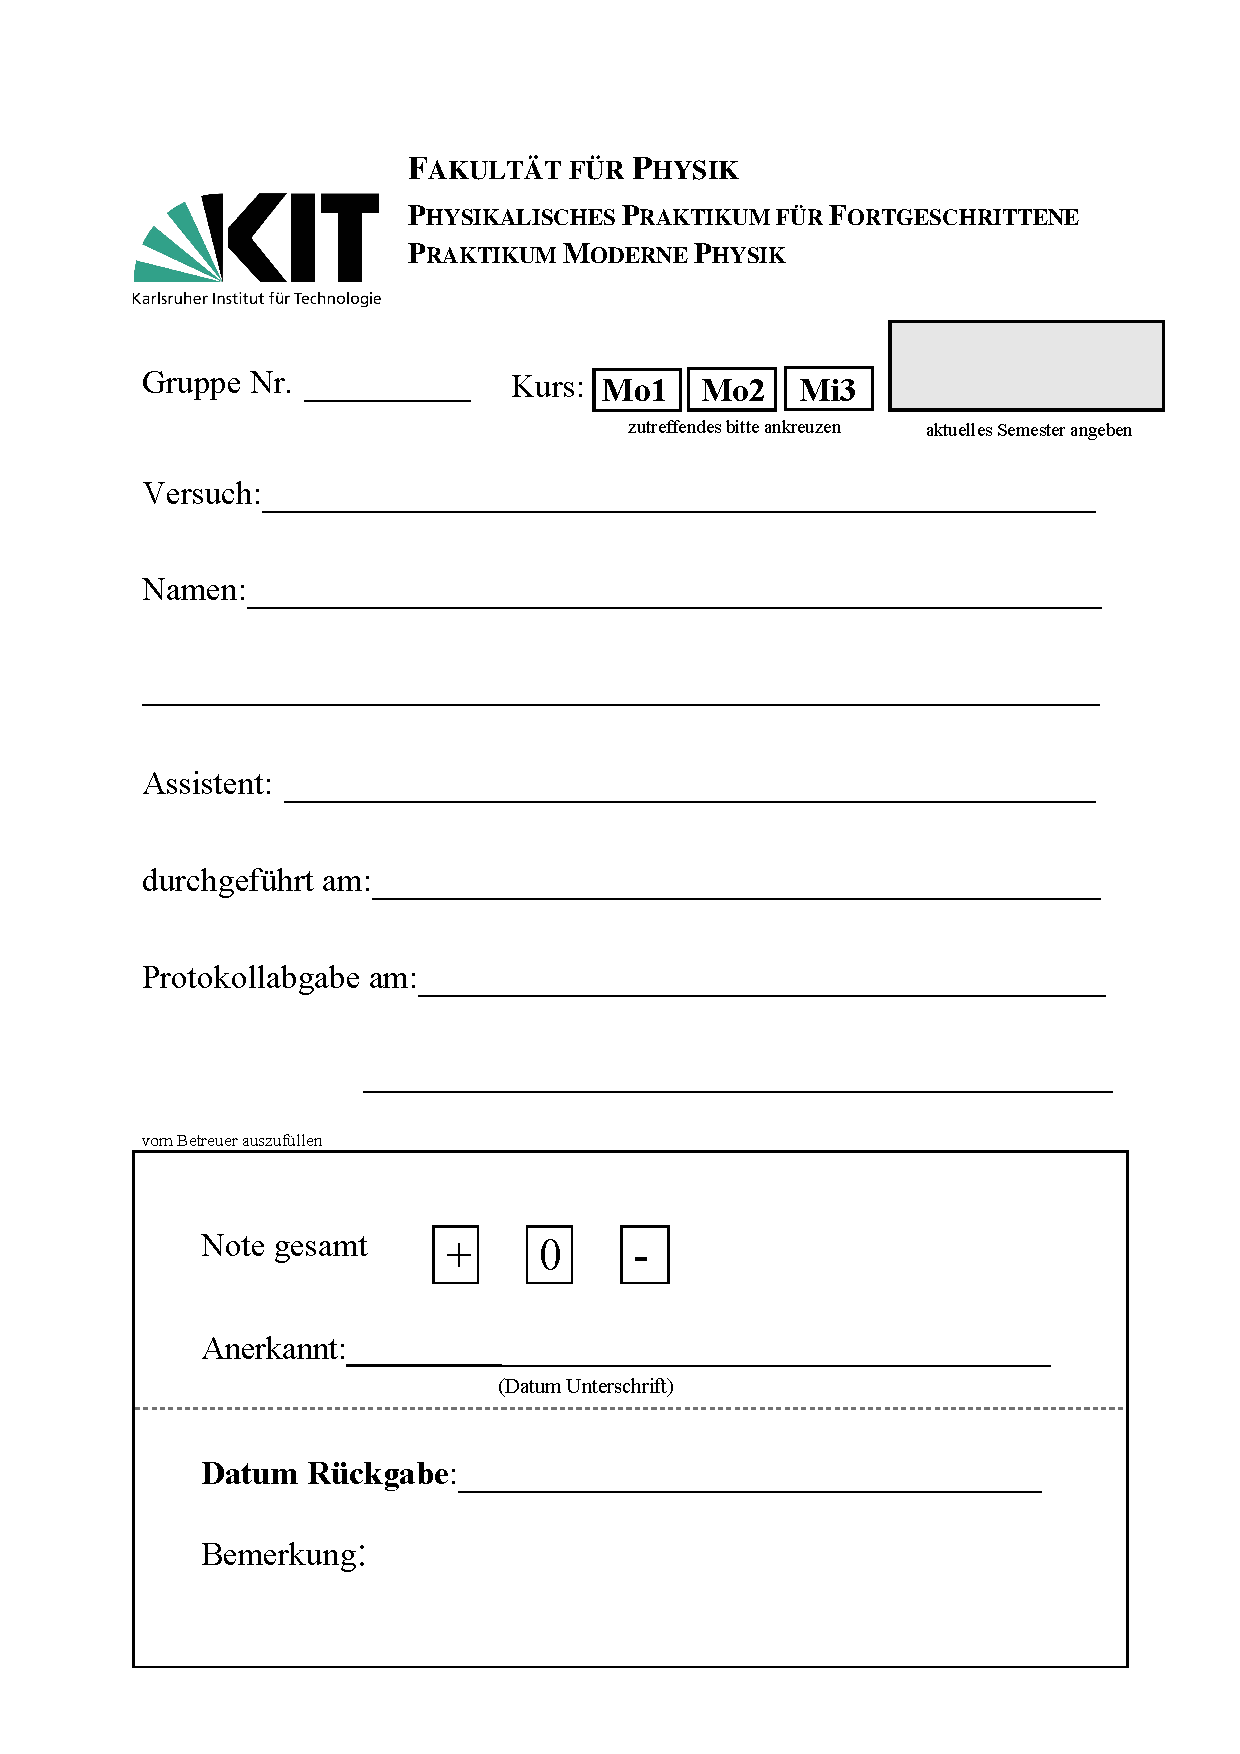
\includegraphics[page=1]{include/DeckblattP3P4.pdf}};
    \begin{scope}[shift={(current page.south west)},every node/.style={anchor=base west}]
        % Grid to help find the positions (remove in final version)
        %\draw [help lines] (0,0) grid (current page.north east);
        %\draw [help lines,thick] (0,0) grid [step=5cm] (current page.north east);
        % Gruppennummer:
        \node at (5.8cm,23.1cm){\Large{\gruppennummer}};
        %Bitte richtigen Wochentag angeben
        %\node at (10 cm,22.8cm) {\scalebox{4}{{$\mathbf{\times}$}}}; % Mo1 Gruppentag:
        %\node at (11.7cm,22.8cm) {\scalebox{4}{{$\mathbf{\times}$}}}; % Mo2 Gruppentag:
        %\node at (13.3 cm,22.8cm) {\scalebox{4}{{$\mathbf{\times}$}}}; % Mi3 Gruppentag:
        \node at (16cm,23.1cm) {\Large{\semester}}; % Semester:
        \node at (4.8cm,21.2cm){\Large{\versuch}}; %Versuch:
        \node at (4.8cm,19.6cm){\Large{\nameeins\hspace{0.2222em}(\emaileins)}}; % Name 1.Zeile:
        \node at (4.8cm,18.0cm){\Large{\namezwei\hspace{0.2222em}(\emailzwei)}}; % Name 2.Zeile:
        \node at (4.8cm,16.3cm){\Large{\assistent}}; % Assistent:in:
        \node at (7.2cm,14.6cm){\Large{\durchfuehrungsdatum}}; % durchgeführt am:
        \node at (7.2cm,13.0cm){\Large{\abgabedatum}}; % Protokollabgabe am:
    \end{scope}
\end{tikzpicture}
% This information will appear embed into the PDF file as meta data
\hypersetup{
  pdftitle    = {\praktikum\hspace{0.2222em}Protokoll - \versuch},
  pdfsubject  = {Protokoll des Versuchs \versuch\hspace{0.2222em}vom \durchfuehrungsdatum},
  pdfauthor   = {\nameeins\hspace{0.2222em}und\hspace{0.2222em}\namezwei\hspace{0.2222em}(Gruppe \gruppentag-\gruppennummer)},
  pdfkeywords = {KIT, Physik, Praktikum, Protokoll, \praktikum, \versuch, \semester, \nameeins, \namezwei},
  pdfcreator  = {pdflatex},
  pdfproducer = {LaTeX with hyperref}
}
%---------------------------------------------%

\newpage
\pagenumbering{arabic} % Ab hier beginnt die Seitennummerierung
\setcounter{page}{1}   % mit Seitenzahl 1. Dies stimmt mit der Seitennummerierung der Aufgabenblätter überein.

%--------Aufgabenblatt----------%
% kann so dem Inhaltsverzeichnis hinzugefügt werden
%\addcontentsline{toc}{chapter}{Aufgabenblatt}

% Im P3&P4 gibt es teilweise keine Aufgabenblatt mehr, sodass dieser Abschnitt auskommentiert werden kann.
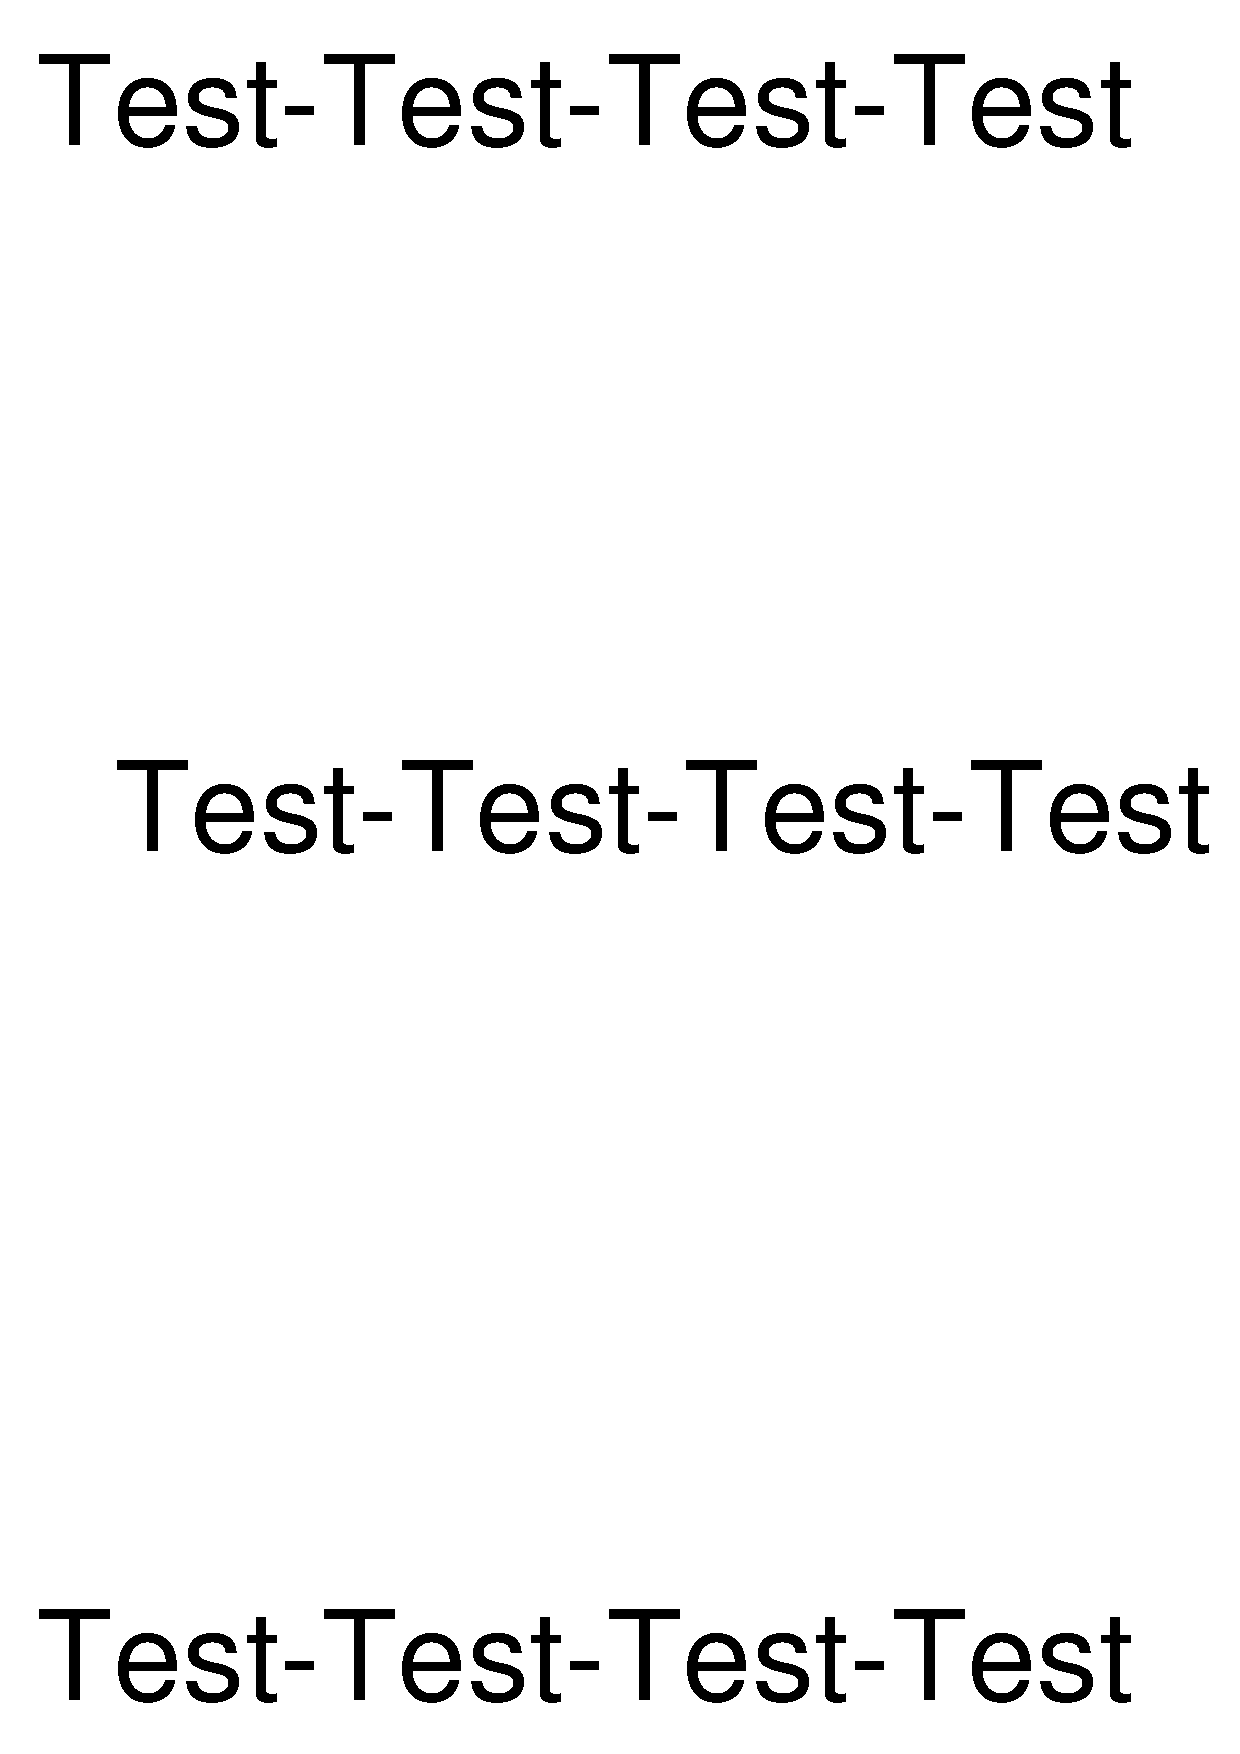
\includepdf[pages=-]{include/Aufgabenblatt.pdf} 
% Die Datei Aufgabenblatt.pdf mit dem Inhalt "Test-Test-Test-Test" muss durch das aktuelle Aufgabenblatt des Versuchs ausgetauscht werden.
%-------------------------------%

%--------Inhaltsverzeichnis, Tabellen- und Abbildungsverzeichnis----------%
\setcounter{chapter}{0} 
% Bei "\setcounter{chapter}{-1}" erhält die Einführung die Kapitelnummer "0";
% Dies kann praktisch sein, um die Kapitelnummer mit den Aufgabennummern der Versuche gleich zu halten.
% Bei "\setcounter{chapter}{0}" startet das Inhaltsverzeichnis bei "1".
\tableofcontents % Erstellt ein Inhaltsverzeichnis
%\vspace{50px}   
%\listoffigures  % Erstellt ein Abbildungsverzeichnis. Dies wird von manchen Tutor:innen gefordert.
%\vspace{50px}   
%\listoftables  % Erstellt ein Tabellenverzeichnis. Dies wird von manchen Tutor:innen gefordert.
\pagebreak
%-------------------------------------------------------------------------%

%--------Inhalt der Kapitel----------%
\input{chapters/Einführung}

\chapter{Theoretische Grundlagen}

\chapter{Experimenteller Aufbau}

\chapter{Durchführung}

\chapter{Auswertung, Fehlerrechnung und Diskussion der Messergebnisse}
%------------------------------------%

%--------Quellen----------%
\newpage
\addcontentsline{toc}{chapter}{Quellen}
\renewcommand{\refname}{Quellen}   
\renewcommand{\bibname}{Quellen} % Lässt die eigene Überschrift des Literaturverzeichnisses verschwinden
\bibliography{include/Quellen.bib}
\bibliographystyle{alphadin}

% use \cite{Example1} to reference
% use \nocite{*} if you want citations to appear even if they are not referenced to.
%-------------------------%

%--------Anhang (Messprotokoll)----------%
\newpage
\addcontentsline{toc}{chapter}{Messprotokoll}
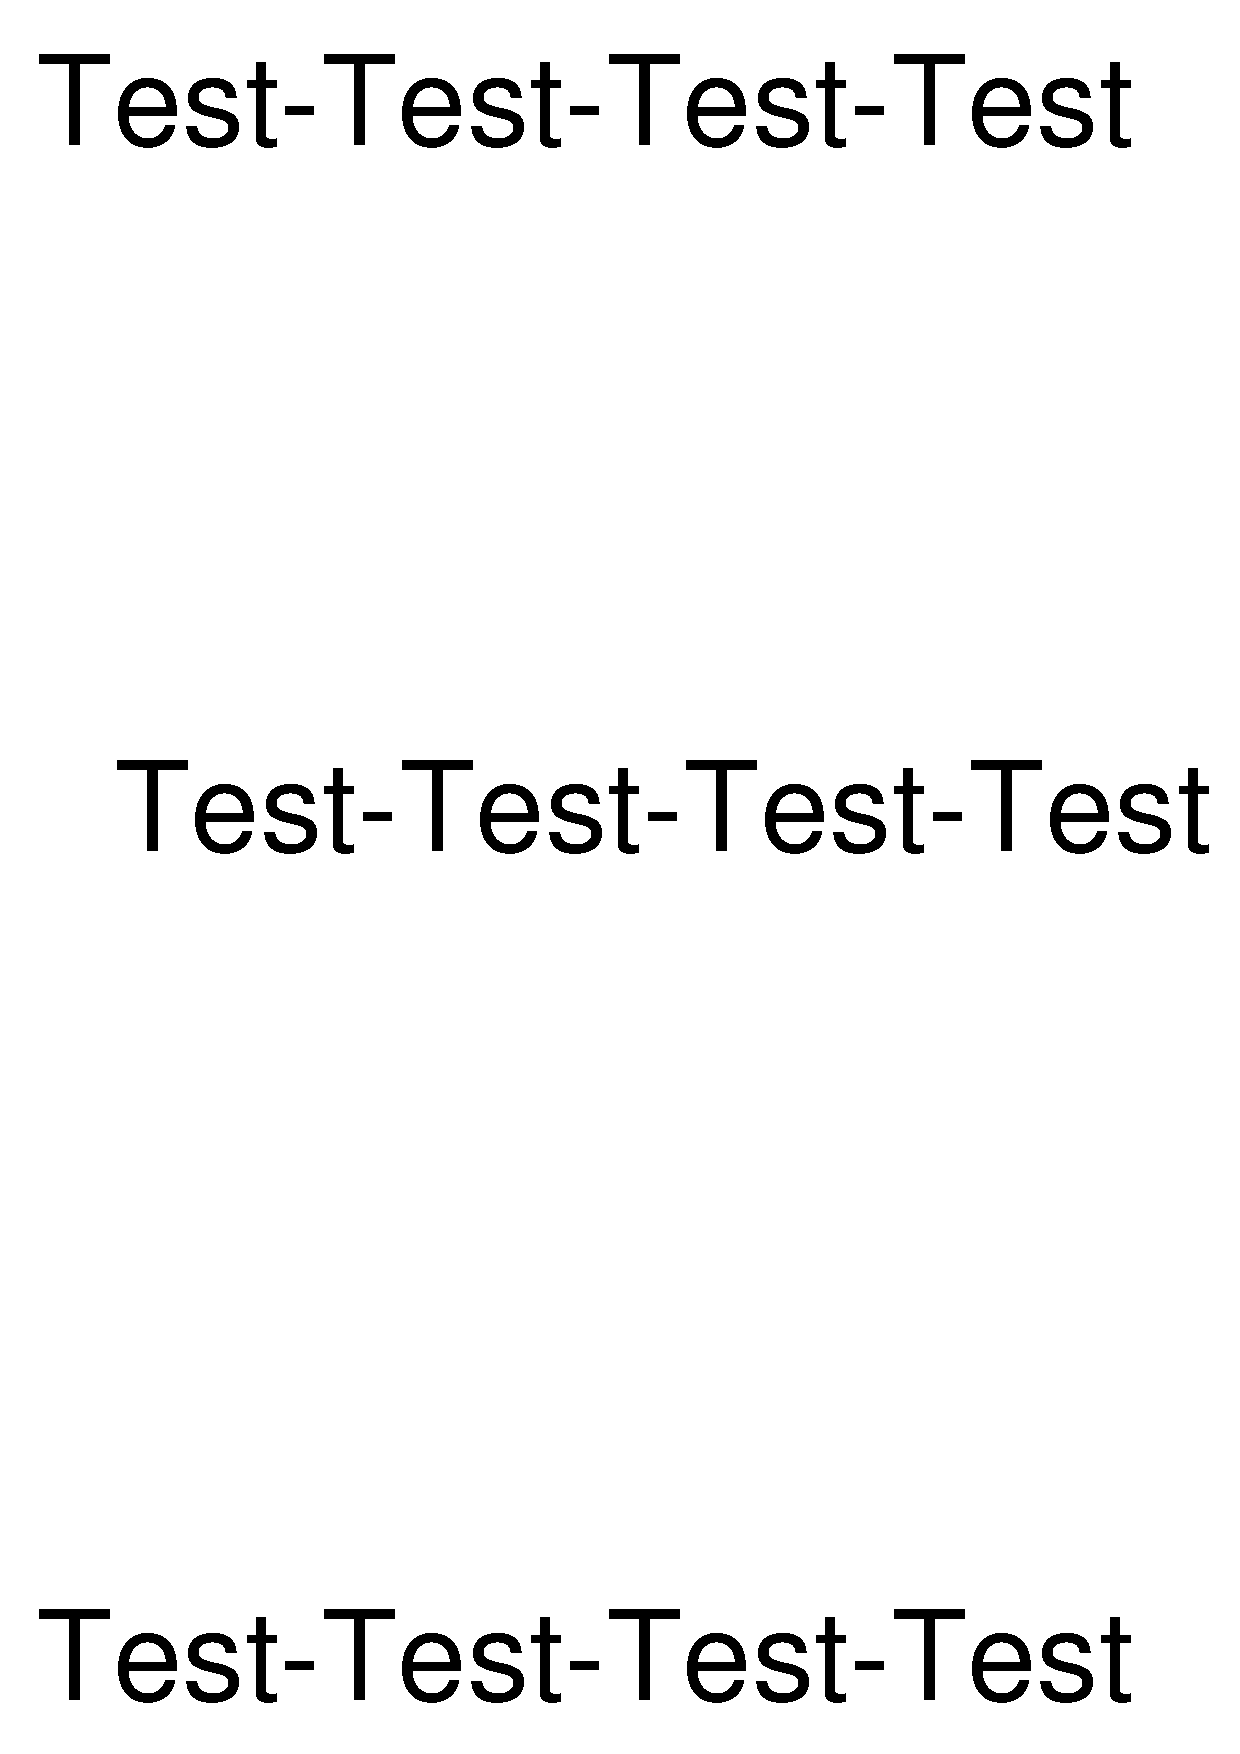
\includepdf[pages=-]{include/Messprotokoll.pdf} 
% Die Datei Messprotokoll.pdf mit dem Inhalt "Test-Test-Test-Test" muss durch das, während des Versuchs erstelltem Messprotokoll, ausgetauscht werden.
%----------------------------------------%

\end{document}